\documentclass{article}
\usepackage{amsmath}
\usepackage[margin=1in]{geometry}
\usepackage{amsfonts}
\usepackage{hyperref}
\usepackage{graphicx}
\usepackage{siunitx}
\usepackage{cancel}

\begin{document}
	
	\title{Gram Schmidt Process}
	\author{Andy Chong Sam}
	
	\maketitle	

\section {Purpose}

\par\noindent The purpose of the Gram Schmidt algorithm is to derive an orthonormal vector set from a list of linearly independent vectors. Given an input set of vectors \(\{\vec v_1, \vec v_2 ... \vec v_n\}\), the algorithm will produce a set \(\{ \hat{u_1}, \hat{u_2} ... \hat{u_n}\}\). Each vector in the output set will be orthogonal to the other members in the set. Finally, both the input and output set will span the same space. 

\section {Algorithm Steps}

\par \noindent Here are the steps, given a set of input vectors \(\{\vec v_1, \vec v_2 ... \vec v_n\}\):

\begin{flalign*}
	\vec u_1 = \vec v_1 \\
	\vec u_2 = \vec v_2 - \text{proj}_{u_1} (v_2) \\
	\vec u_3 = \vec v_3 - \text{proj}_{u_1} (v_3) - \text{proj}_{u_2} (v_3) 
\end{flalign*}

\par \noindent We can generalize \(\vec u_n\):

\begin{flalign*}
	\vec u_n = \vec v_k - \sum_{j=1}^{k-1} \text{proj}_{u_j} (v_k) 
\end{flalign*}

\par \noindent We conclude with normalizing \(\vec u_1\), \(\vec u_2\), ... \(\vec u_n\) to obtain the orthonormal set: 

\begin{flalign*}
	 \{\frac{\vec u_1}{|| \vec u_1 ||},\frac{\vec u_2}{|| \vec u_2 ||},\frac{\vec u_3}{|| \vec u_3 ||} ... \frac{\vec u_n}{|| \vec u_n ||} \} =
	\{ \hat{u_1}, \hat{u_2} ... \hat{u_n}\}
\end{flalign*}


\section {Intuition Using Two Vectors}

\par \noindent Figure (1) shows the geometric intuition using two vectors in \(\mathbb{R}^2\):
\newline
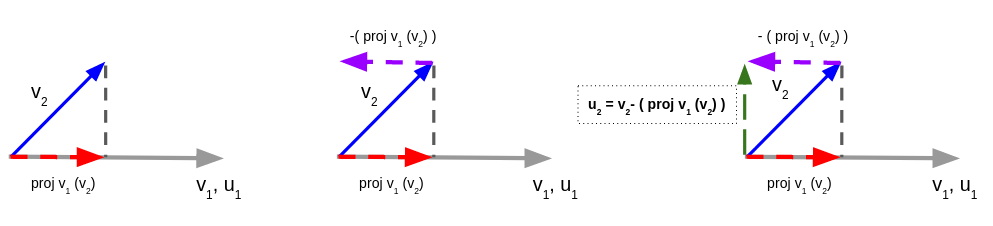
\includegraphics[width=17cm]{gs-2d.png}	
\begin{center}
	Figure 1
\end{center}
\newpage
\par \noindent  If \( \hat{u_1}\) and \(\hat{u_2}\) are orthogonal to each other, then their dot product is zero. Suppose that \(\vec v_1=<a,b>\) and \(\vec v_2=<c,d>\). The first vector is just \(\vec v_1\). 
\newline
\par \noindent We now calculate \(\vec u_2\):

\begin{flalign*}
<c,d> - (\frac{ac + bd}{a^2 + b^2}<a,b>)
\end{flalign*}

\par\noindent We can now take this result and perform a dot product with \(\vec v_1\):

\begin{flalign*}
	(<c,d> - (\frac{ac + bd}{a^2 + b^2}<a,b>))\cdot <a,b> \\
	= a(c- \frac{ac+bd}{a^2+b^2}a) + b(d-\frac{ac+bd}{a^2+b^2}b)\\
	= ac - a^2\frac{ac+bd}{a^2+b^2} + bd - b^2\frac{ac+bd}{a^2+b^2} \\
	=\frac{ac(a^2+b^2)}{a^2+b^2} - \frac{a^2(ac+bd)}{a^2+b^2} + \frac{bd(a^2+b^2)}{a^2+b^2} - \frac{b^2(ac+bd)}{a^2+b^2}\\
	= \frac{a^3c+ab^2c-a^3c-a^2bd+a^2bd+b^3d-ab^2c-b^3d}{a^2+b^2} \\
	= 0
\end{flalign*}

\framebox{
	\parbox{\linewidth}{
		\textbf{Ex. 1} Given \(\vec v_1 = <3,1>\) and \(\vec v_2 = <2,2>\) find an orthonormal set using the Gram Schmidt process.
		\newline
		\par\noindent We have \(\vec u_1 = \vec v_1\), so \( \vec u_1 = <3,1>\).
		\newline
		\par\noindent We proceed to derive \( \vec u_2 \):
		\begin{flalign*}
			\vec u_2 = \vec v_2 - \text{proj}_{u_1} (v_2) \\
			= <2,2> - (\; \frac{(3)(2)+ (1)(2)}{(3)(3)+(1)(1)}<3,1> \;) \\
			= <2,2> - \frac{4}{5}<3,1>\\
			= <\frac{-2}{5},\frac{6}{5}>
		\end{flalign*}
		\par \noindent To conclude, normalize \(\vec u_1\) and \(\vec u_2\). We find that \( || \vec u_1 || = \sqrt{10}\) and \( || \vec u_2 || = \sqrt{\frac{8}{5}}\), so the orthonornmal set is:
		\begin{flalign*}
			\hat{u_1} = \frac{1}{\sqrt{10}}<3,1> \\
			\hat{u_2} = \frac{\sqrt{5}}{\sqrt{8}} <\frac{-2}{5}, \frac{6}{5}>
		\end{flalign*}
		\par\noindent This result can be verified by showing that \(\hat{u_1} \cdot \hat{u_2}\) is zero:
		\begin{flalign*}
			(\frac{3}{\sqrt{10}})(\frac{\sqrt{5}}{\sqrt{8}})(\frac{-2}{5}) + (\frac{1}{\sqrt{10}})(\frac{\sqrt{5}}{\sqrt{8}})(\frac{6}{5})	= 0
		\end{flalign*}
}}
\newpage
\framebox{
	\parbox{\linewidth}{
		\textbf{Ex. 2} Given \(\vec v_1 = <1,2,0>\) and \(\vec v_2 = <8,1,-6>\) and \(\vec v_3 = <0,0,1>\) find an orthonormal set using the Gram Schmidt process:
		\newline
		\par\noindent We have \(\vec u_1 = \vec v_1\), so \( \vec u_1 = <1,2,0>\).
		\newline
		\par\noindent Let's calculate \( \vec u_2\): 
		\begin{flalign*}
				\vec u_2 = \vec v_2 - \text{proj}_{u_1} (v_2)
		\end{flalign*}
		\begin{flalign*}		
			\vec u_2  = <8,1,-6> - \frac{(1)(8) + (2(1) + (0)(-6)}{(1)(1) + (2)(2) + (0)(0)}<1,2,0>\\
			=<6,-3,-6>
		\end{flalign*}
		\par\noindent Let's calculate \( \vec u_3\):
		
		\begin{flalign*}
\vec u_3 = \vec v_3 - \text{proj}_{u_1} (v_3) - \text{proj}_{u_2} (\vec v_3)
		\end{flalign*}
		
		
		\begin{flalign*}
		\vec u_3 = <0,1,1> - \frac{(1)(0) + (2)(0) + (0)(1)}{(1)(1) + (2)(2) + (0)(0)}<1,2,0> - \frac{(1)(8)+(2)(1) + (0)(0)}{(6)(6) + (-3)(-3) + (-6)(-6)}<6,-3,-6> \\
	= <\frac{4}{9}, -\frac{2}{9}, \frac{5}{9}>	
	\end{flalign*}
	
		\par \noindent We conclude with normalizing our results given that \( || \vec u_1 || = \sqrt{5}\), \( || \vec u_2 || = 9\), and \( || \vec u_3 || = \frac{\sqrt{45}}{9}\):
		
		\begin{flalign*}
			\hat{u_1} = \frac{1}{\sqrt{5}} = <1,2,0> \\
			\hat{u_2} = \frac{1}{3}<6,-3,-6> \\
			\hat{u_3} =  \frac{1}{\sqrt{45}} <4, -2, 5>
		\end{flalign*}
	
	
		
}}
\end{document}